\documentclass[aspectratio=169]{beamer}
\usepackage{graphicx} % Required for inserting images

\usepackage{tikz}

\usetheme{Madrid}

\usetheme{Antibes}

\definecolor{rojoUGR}{HTML}{d53044}
\definecolor{darkgray}{HTML}{737572}
\definecolor{text}{HTML}{99a6ad}
\definecolor{lightgray}{gray}{0.95}


\definecolor{lavendergray}{rgb}{0.77, 0.76, 0.82}
\colorlet{beamer@blendedblue}{rojoUGR}

\setbeamercolor{normal text}{fg=darkgray}
\setbeamercolor{block title}{bg=darkgray}
\setbeamercolor{block body}{bg=white}
%\setbeamercolor{structure}{fg=rojoUGR}
%\colorlet{beamer@blendedblue}{rojoUGR}

% This is for using different fonts
\usepackage[sfdefault]{roboto}  %% Option 'sfdefault' only if the base font of the document is to be sans serif
\usepackage[T1]{fontenc}

%Color de los bulltets
\setbeamertemplate{itemize item}[square]
\setbeamercolor{itemize item}{fg=darkgray}
\setbeamertemplate{itemize subitem}[circle]
\setbeamercolor{itemize subitem}{fg=darkgray}
\setbeamercolor{itemize subsubitem}{fg=darkgray}
\setbeamertemplate{itemize subsubitem}[square]
\setbeamercolor{enumerate item}{fg=darkgray}
\setbeamertemplate{enumerate item}[square]

% Para añadir subtitulos a las diapositivas
\setbeamercolor{framesubtitle}{fg=darkgray}
\setbeamerfont{framesubtitle}{size=\small,series=\itshape}

%remove navigation symbols
\setbeamertemplate{navigation symbols}{}

%remove headline tree
\setbeamertemplate{headline}{}

%% Modificar el pie de página para que se asemeje al de la UGR
\setbeamertemplate{footline}[text line]{LaTeX Avanzado}
\setbeamertemplate{footline}{%
                \hspace{0.5cm}%
                \vspace{0.2cm}%
                
\includegraphics[height=0.6cm]{imagenes/nuevoPollo2.png}%
                \hfill
                \rule[0.3cm]{\dimexpr\linewidth-2cm\relax}{0.4pt}%
                \hfill
                \usebeamercolor[fg]{page number in head/foot}%
                \usebeamerfont{page number in head/foot}%
                \raisebox{0.25cm}{%
                    \tikz[baseline=(char.base)]{
                        \node[shape=circle, fill=rojoUGR, text=white, inner sep=2pt] (char) {\insertframenumber};
                    }
                }\,\kern2em%
}

%% Modificar el título para que se asemeje al de la UGR
\setbeamercolor{frametitle}{fg=rojoUGR}
\setbeamertemplate{frametitle}{%
    \vspace{0.2cm}%
    \begin{tikzpicture}[baseline=(title.base)]
        % Línea vertical
        \node[anchor=base west] (line) at (0,1cm) {\tikz[baseline] \draw[darkgray, line width=3pt] (0,-0.08cm) -- (0,-1.0cm);};
        % Título al lado de la línea
        \node[anchor=base west] (title) at ([xshift=0.0cm, yshift=0.05cm]line.east) {%
            \usebeamercolor[fg]{frametitle}%
            \usebeamerfont{frametitle}\insertframetitle%
        };
        % Subtítulo debajo del título, alineado con la línea
        \node[anchor=north west] (subtitle) at ([yshift=0.2cm]title.south west) {%
            \usebeamercolor[fg]{framesubtitle}%
            \usebeamerfont{framesubtitle}\insertframesubtitle%
        };
    \end{tikzpicture}%
    \vspace{0.2cm}%
}


\usepackage[spanish]{babel}

\usepackage{lmodern}

%Para poder usar las tildes. Hay que guardar el documento en uft-8
\usepackage[utf8]{inputenc}

\usepackage{amsmath}

\usepackage{mathtools}

%Para usar columnas
\usepackage{multicol}
\usepackage{multirow}
\usepackage{booktabs}
\usepackage{listings}

\usepackage{amsmath}


\usepackage{graphicx} % Required for inserting images

\usepackage{tikz}

\usetheme{Antibes}

\definecolor{rojoUGR}{HTML}{d53044}
\definecolor{darkgray}{HTML}{737572}
\definecolor{text}{HTML}{99a6ad}
\definecolor{lightgray}{gray}{0.95}


\definecolor{lavendergray}{rgb}{0.77, 0.76, 0.82}
\colorlet{beamer@blendedblue}{rojoUGR}

\setbeamercolor{normal text}{fg=darkgray}
\setbeamercolor{block title}{bg=darkgray}
\setbeamercolor{block body}{bg=white}
%\setbeamercolor{structure}{fg=rojoUGR}
%\colorlet{beamer@blendedblue}{rojoUGR}

% This is for using different fonts
\usepackage[sfdefault]{roboto}  %% Option 'sfdefault' only if the base font of the document is to be sans serif
\usepackage[T1]{fontenc}

%Color de los bulltets
\setbeamertemplate{itemize item}[square]
\setbeamercolor{itemize item}{fg=darkgray}
\setbeamertemplate{itemize subitem}[circle]
\setbeamercolor{itemize subitem}{fg=darkgray}
\setbeamercolor{itemize subsubitem}{fg=darkgray}
\setbeamertemplate{itemize subsubitem}[square]
\setbeamercolor{enumerate item}{fg=darkgray}
\setbeamertemplate{enumerate item}[square]

% Para añadir subtitulos a las diapositivas
\setbeamercolor{framesubtitle}{fg=darkgray}
\setbeamerfont{framesubtitle}{size=\small,series=\itshape}

%remove navigation symbols
\setbeamertemplate{navigation symbols}{}

%remove headline tree
\setbeamertemplate{headline}{}

%% Modificar el pie de página para que se asemeje al de la UGR
\setbeamertemplate{footline}[text line]{LaTeX Avanzado}
\setbeamertemplate{footline}{%
                \hspace{0.5cm}%
                \vspace{0.2cm}%
                
\includegraphics[height=0.6cm]{imagenes/nuevoPollo2.png}%
                \hfill
                \rule[0.3cm]{\dimexpr\linewidth-2cm\relax}{0.4pt}%
                \hfill
                \usebeamercolor[fg]{page number in head/foot}%
                \usebeamerfont{page number in head/foot}%
                \raisebox{0.25cm}{%
                    \tikz[baseline=(char.base)]{
                        \node[shape=circle, fill=rojoUGR, text=white, inner sep=2pt] (char) {\insertframenumber};
                    }
                }\,\kern2em%
}

%% Modificar el título para que se asemeje al de la UGR
\setbeamercolor{frametitle}{fg=rojoUGR}
\setbeamertemplate{frametitle}{%
    \vspace{0.2cm}%
    \begin{tikzpicture}[baseline=(title.base)]
        % Línea vertical
        \node[anchor=base west] (line) at (0,1cm) {\tikz[baseline] \draw[darkgray, line width=3pt] (0,-0.08cm) -- (0,-1.0cm);};
        % Título al lado de la línea
        \node[anchor=base west] (title) at ([xshift=0.0cm, yshift=0.05cm]line.east) {%
            \usebeamercolor[fg]{frametitle}%
            \usebeamerfont{frametitle}\insertframetitle%
        };
        % Subtítulo debajo del título, alineado con la línea
        \node[anchor=north west] (subtitle) at ([yshift=0.2cm]title.south west) {%
            \usebeamercolor[fg]{framesubtitle}%
            \usebeamerfont{framesubtitle}\insertframesubtitle%
        };
    \end{tikzpicture}%
    \vspace{0.2cm}%
}

% \usetheme{Antibes}
% \usecolortheme{beaver}

%Para poder usar las tildes. Hay que guardar el documento en uft-8
\usepackage[utf8]{inputenc}

%Para incluir código fuente
\usepackage{lstautogobble}
\usepackage{listings}
\lstset{
    language=[LaTeX]TeX,
    texcsstyle=*\bf\color{blue},
     basicstyle=\tiny\ttfamily, frame=single, columns=fullflexible,
     breaklines=false, showtabs=false, upquote=true, showstringspaces=false,
      keywordstyle=\color{blue}, commentstyle=\color{red}, stringstyle=red,
      numberstyle=\tiny\color{mygray, autogobble=true}
}

\title{LLM COMO SERVICIO}



\subtitle{\textit{MiIA UGR (Mi Inteligencia Artificial)}}
\author{Isaac Vidal Daza}
\institute{Apoyo a la Docencia \newline Centro de Servicios de Informática y Redes de Comunicaciones \newline Universidad de Granada}
\date{22-05-2025}

% logo of my university


\titlegraphic{
   
\includegraphics[width=4cm,align=c]{imagenes/logoCSIRCDef.png}
    
\includegraphics[height=0.6cm, align=c]{imagenes/redIris.png} 
}


\setbeamertemplate{footline}{%
        \hspace{0.5cm}%
        \vspace{0.2cm}%
        
\includegraphics[align=r, height=0.8cm]{imagenes/nuevoPollo2.png}%
        \hfill%
        
\includegraphics[height=1cm, align=c]{imagenes/redIris.png}
        %\textit{JJTT RedIRIS 2025}
        \usebeamercolor[fg]{page number in head/foot}%
        \usebeamerfont{page number in head/foot}%
        \insertframenumber\,/\,\inserttotalframenumber\kern1em%
 }

% Listing
%Para incluir código fuente
\usepackage{listings}
\lstset{ 
     basicstyle=\scriptsize\ttfamily, frame=single, columns=fullflexible,
     breaklines=true, showtabs=false, upquote=true, showstringspaces=false,
      keywordstyle=\color{blue}, numberstyle=\tiny\color{darkgray}
}

\begin{document}

\begin{frame}
    %\titlepage
    \maketitle
\end{frame}
%

%
%Sección Introducción

\begin{frame}{Inteligencia Artificial (según los "Mass Media")}

    \begin{center}
        
\includegraphics[width=9cm]{imagenes/final_trick.png}
    \end{center}

\end{frame}

\begin{frame}{Modelos de Lenguaje}

    \begin{block}{Lámpara Mágica}
        \begin{center}
            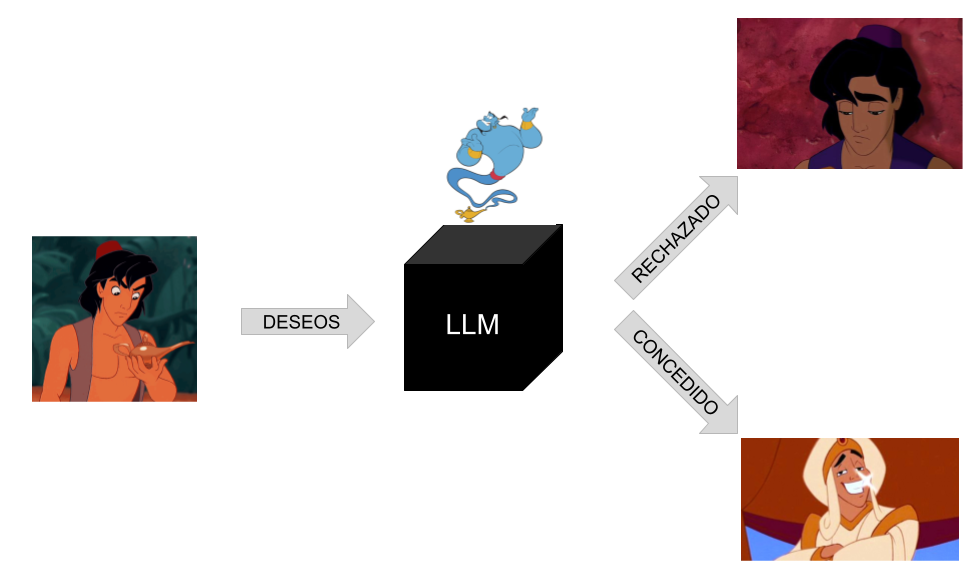
\includegraphics[width=10cm]{imagenes/llm-blacbox.png}
        \end{center}
    \end{block}

\end{frame}


\begin{frame}{Core MiIA}
    \framesubtitle{Componentes del Servicio}

    \begin{center}
        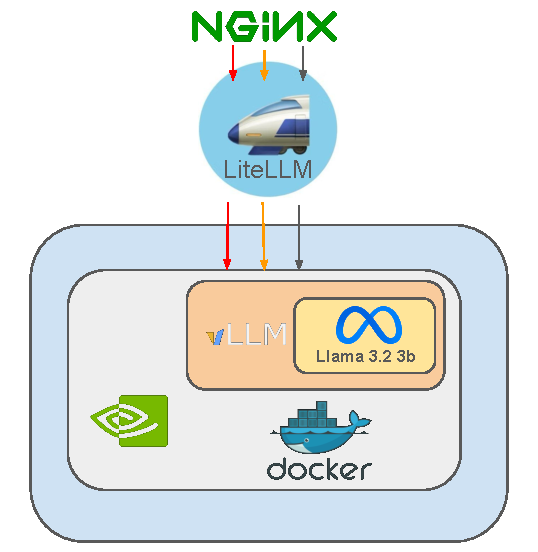
\includegraphics[height=6cm]{imagenes/MiIA_core.pdf}
    \end{center}


\end{frame}

\begin{frame}{LiteLLM: proxy LLM}
    \framesubtitle{Definición de API keys: \textit{Virtual Keys}}

    \begin{center}
        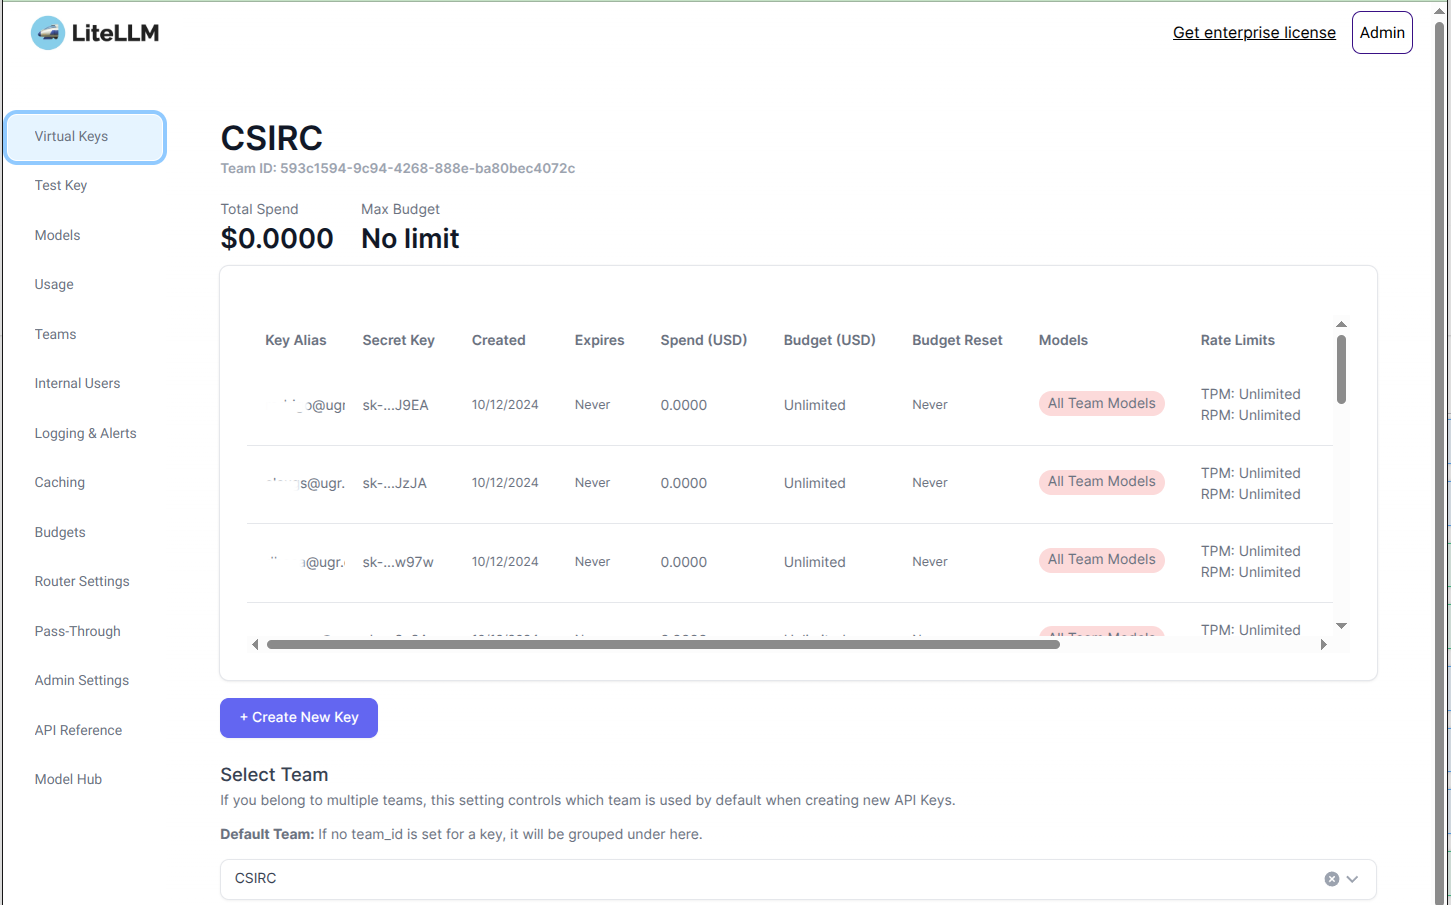
\includegraphics[height=6cm]{imagenes/LiteLLM_vkeys.png}
    \end{center}

\end{frame}

\begin{frame}{LiteLLM: proxy LLM}
    \framesubtitle{Definición de modelos y control de accesos.}

    \begin{center}
        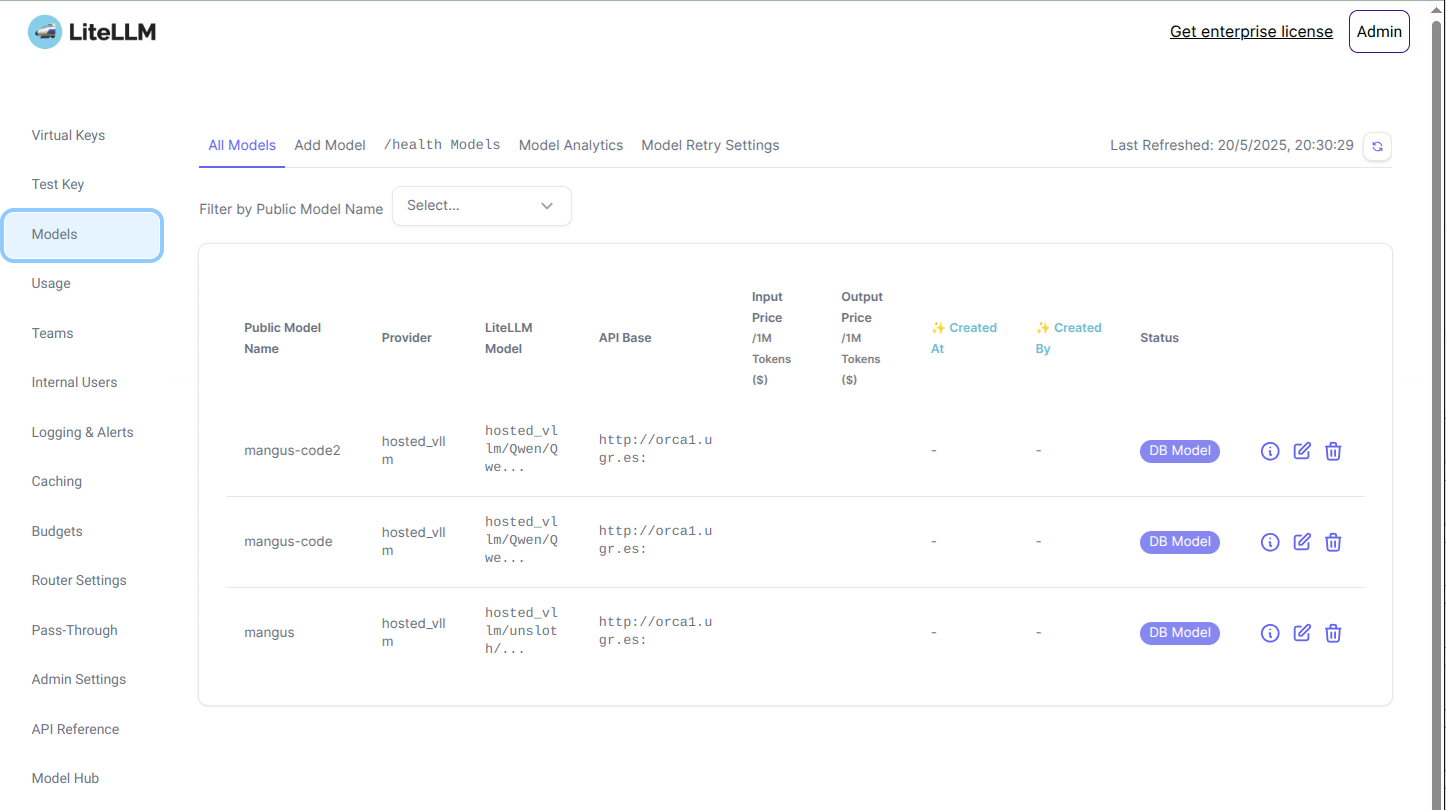
\includegraphics[height=6cm]{imagenes/LiteLLM_models.png}
    \end{center}

\end{frame}

\begin{frame}{LiteLLM: proxy LLM}
    \framesubtitle{Escalado del servicio LLM}

    \begin{center}
        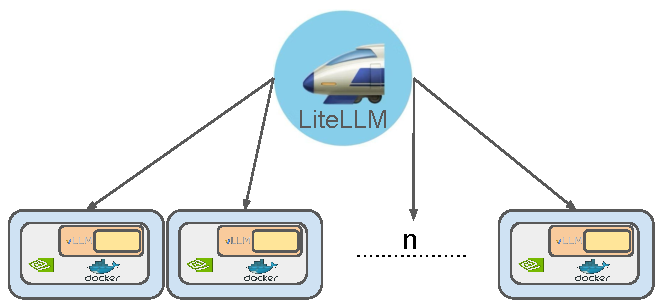
\includegraphics[height=6cm]{imagenes/LiteLLM_scaling.pdf}
    \end{center}

\end{frame}

\begin{frame}{Core MiIA}
    \framesubtitle{Componentes del Servicio}

    \begin{center}
        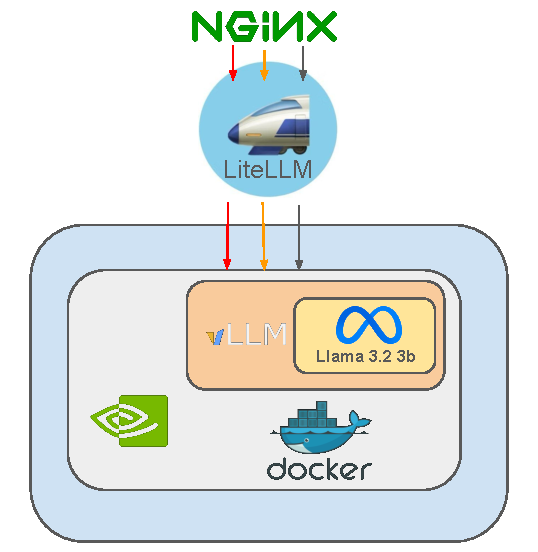
\includegraphics[height=6cm]{imagenes/MiIA_core.pdf}
    \end{center}

\end{frame}

\begin{frame}{vLLM}
    \framesubtitle{Servidor de Inferencia}

    \begin{center}
        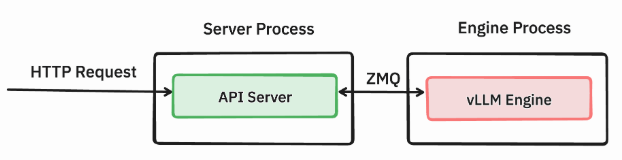
\includegraphics[height=4cm]{imagenes/vllm_arch.png}
    \end{center}

\end{frame}

\begin{frame}{Servicios Ofrecidos con MiIA Core}
    \framesubtitle{MiIA Chat (\textbf{Open WebUI})}

    \begin{center}
        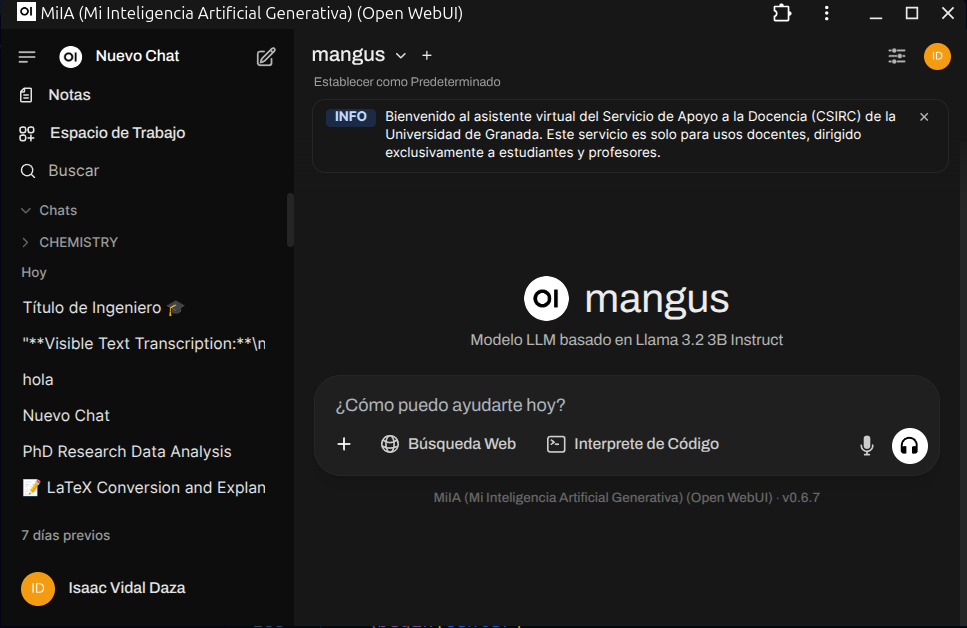
\includegraphics[height=6cm]{imagenes/MiIA_chat.png}
    \end{center}

\end{frame}

\begin{frame}{Servicios Ofrecidos con MiIA Core}
    \framesubtitle{MiIA Chat (\textbf{Open WebUI}): Arquitectura}

    \begin{center}
        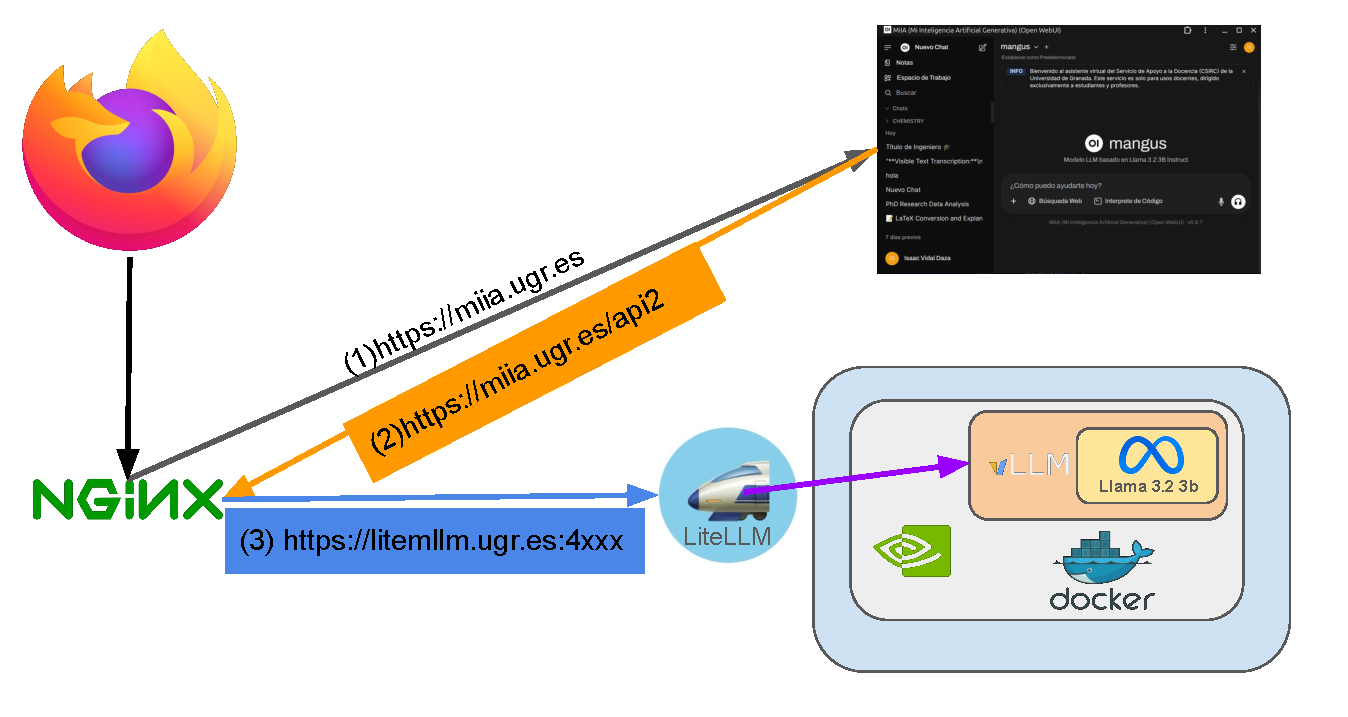
\includegraphics[height=6cm]{imagenes/MiIA_chat_arch.pdf}
    \end{center}

\end{frame}

\begin{frame}{Servicios Ofrecidos con MiIA Core}
    \framesubtitle{\textbf{ThunderAI}: Extensión de Thunderbird para correo electrónico}

    \begin{center}
        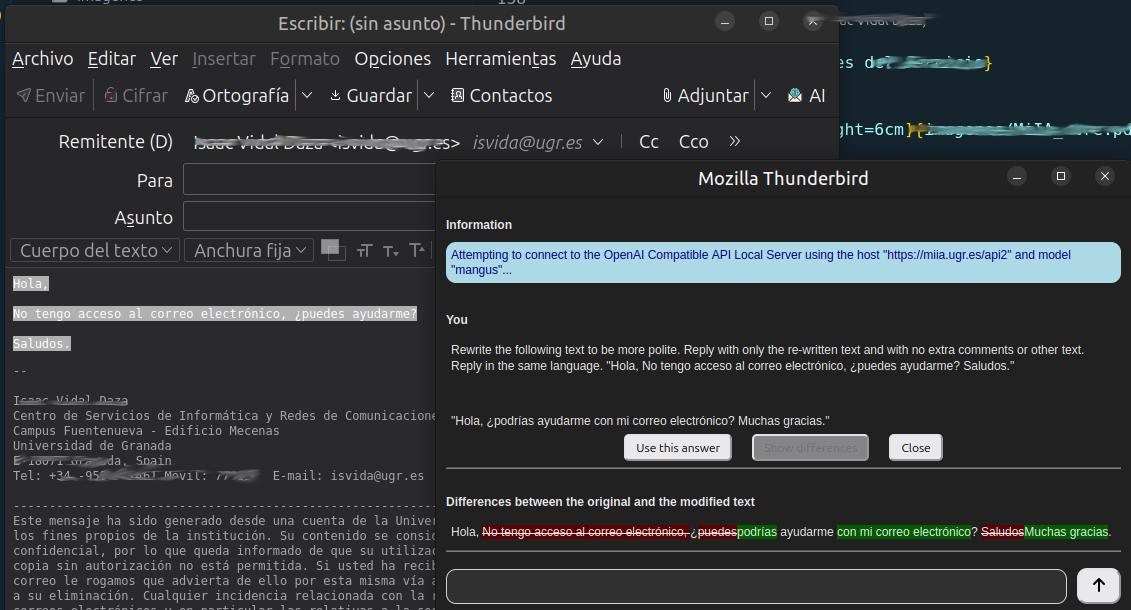
\includegraphics[height=6cm]{imagenes/thunderAI.png}
    \end{center}

\end{frame}


\begin{frame}{Servicios Ofrecidos con MiIA Core}
    \framesubtitle{\textbf{Continue}: Extensión de Visual Studio Code para desarrollo asistido por IA}

    \begin{center}
        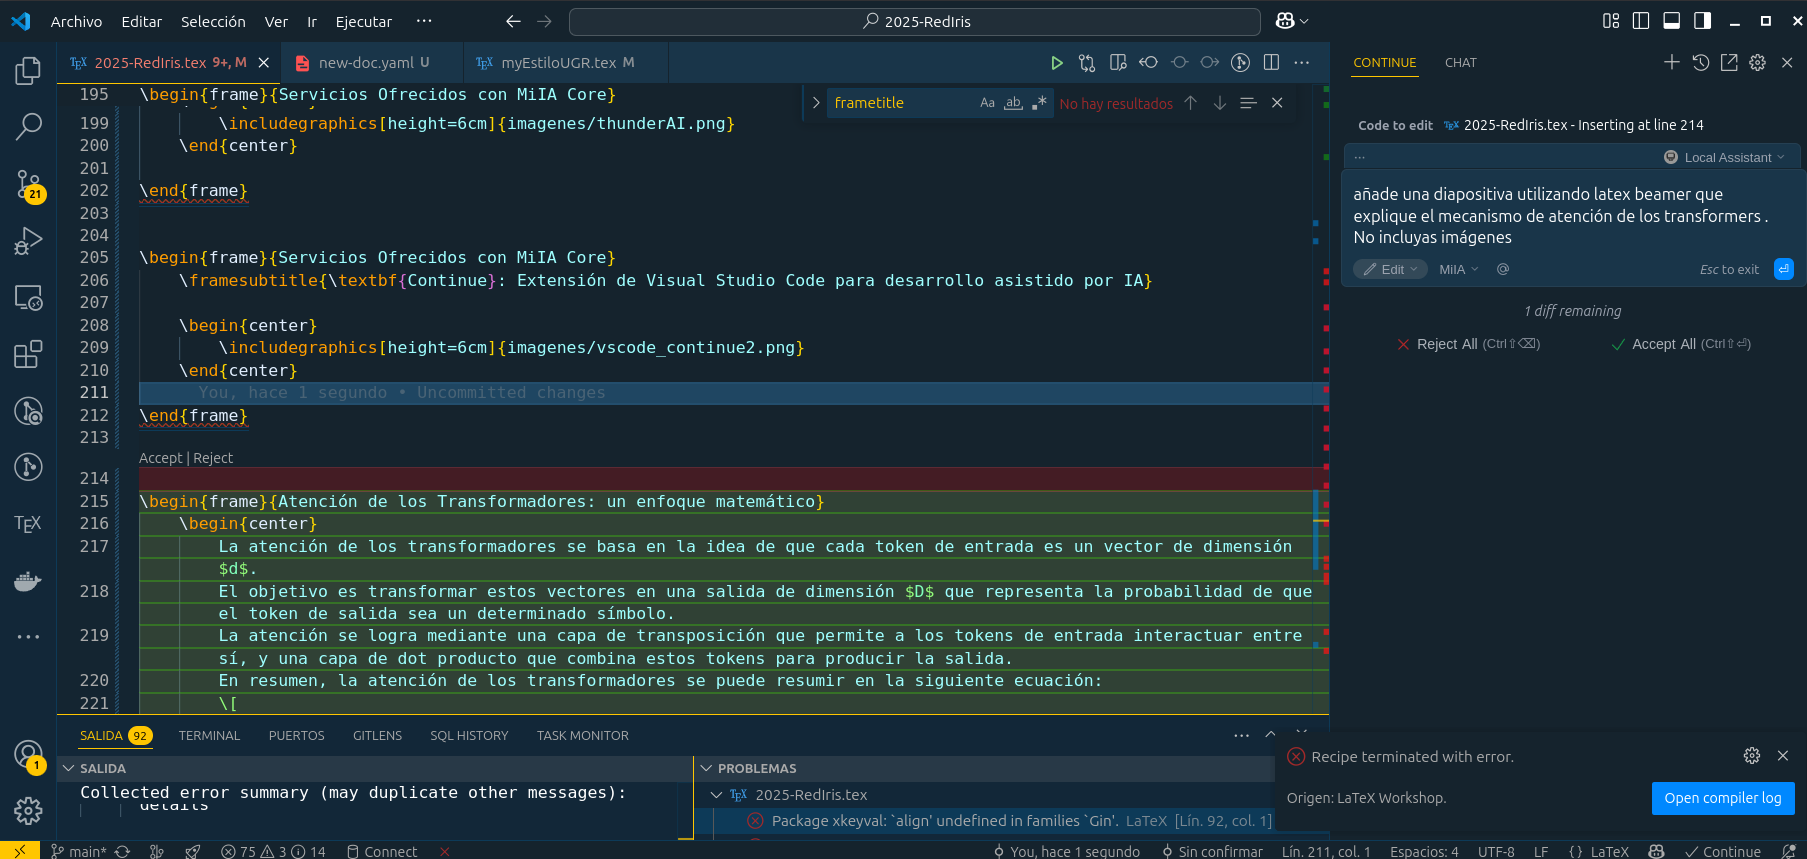
\includegraphics[height=6cm]{imagenes/vscode_continue3.png}
    \end{center}

\end{frame}

\begin{frame}{Atención de los Transformadores: un enfoque matemático}
    \begin{center}
        La atención de los transformadores se basa en la idea de que cada token de entrada es un vector de dimensión $d$.
        El objetivo es transformar estos vectores en una salida de dimensión $D$ que representa la probabilidad de que el token de salida sea un determinado símbolo.
        La atención se logra mediante una capa de transposición que permite a los tokens de entrada interactuar entre sí, y una capa de dot producto que combina estos tokens para producir la salida.
        En resumen, la atención de los transformadores se puede resumir en la siguiente ecuación:
        \[
        \text{Output} = \sum_{i=1}^{L} \text{Attention}(i) \times \text{Output}_i
        \]
        donde $\text{Attention}(i)$ es la atención dada por el token $i$ y $\text{Output}_i$ es el output del token $i$.
    \end{center}
\end{frame}

\begin{frame}{Reconocimiento (\textit{Parseo}) de Documentos}
    \framesubtitle{Carrera Horizontal del PTGAS}
    \begin{itemize}
        \item Entrega de documentación para la evaluación.
        \item Análisis de 11510 documentos en poco tiempo.
    \end{itemize}
    \begin{center}
        
\includegraphics[width=8cm]{imagenes/cienciaDatos.png}
    \end{center}
\end{frame}

\begin{frame}{Reconocimiento (\textit{Parseo}) de Documentos}
    \framesubtitle{EPFReader}
        \begin{center}
            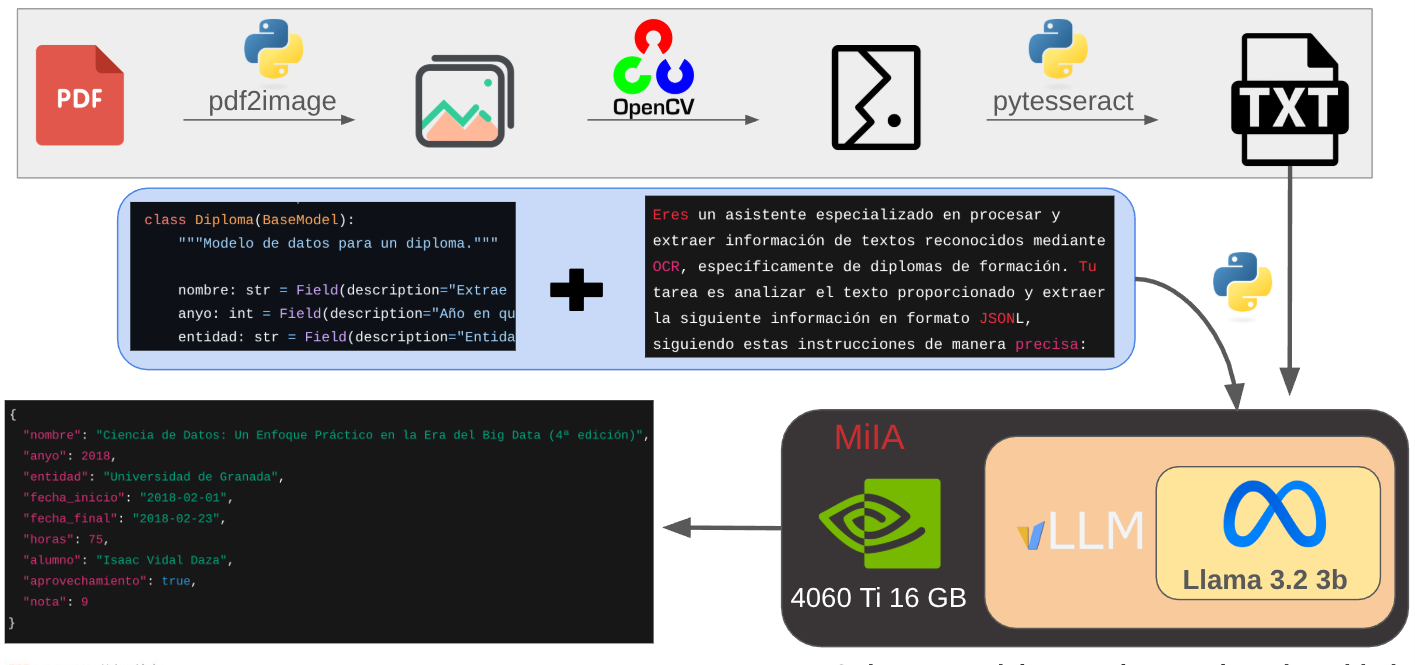
\includegraphics[width=12cm]{imagenes/epf.png}
        \end{center}
\end{frame}

\begin{frame}
        \begin{center}
            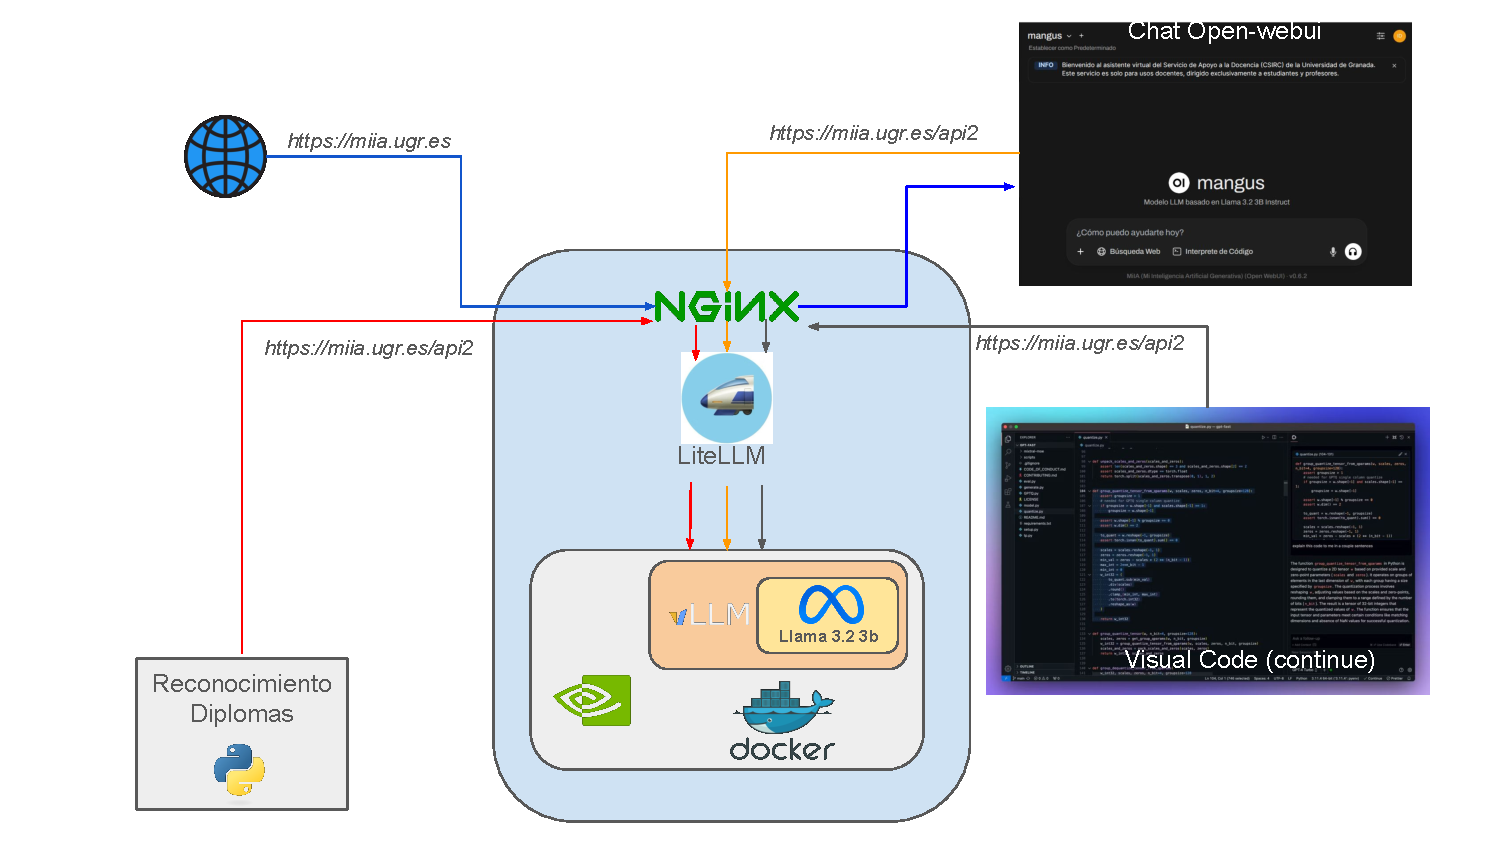
\includegraphics[width=14cm]{imagenes/MiIA_completo.pdf}
        \end{center}
\end{frame}


\begin{frame}{Servicio de Apoyo a la Docencia}
    \begin{block}{\centering Personal}
        \begin{columns}
            \begin{column}{0.5\linewidth}

                \begin{itemize}
                    \item Francisco Romera Juárez. (Head)
                    \item Fernando López Álvarez.
                    \item Antonio Cano Ruano.
                \end{itemize}

            \end{column}
            \begin{column}{0.5\linewidth}
                \begin{itemize}
                    \item Rodrigo González Gálvez.
                    \item Domingo Baca Ruíz.
                    \item Leire Melchor López.
                    \item Isaac Vidal Daza.
                \end{itemize}
            \end{column}
        \end{columns}
    \end{block}
\end{frame}


\begin{frame}{Preguntas}
    \begin{block}{Presentación y Código}
    \begin{center}
        \href{https://github.com/isvida/2025-RedIris}{https://github.com/isvida/2025-RedIris}
    \end{center}
\end{block}
\end{frame}




\end{document}